\chapter{Probability Distributions}

%
% TODO:  Students were confused about how to handle bin position
% for plotting discrete data...  some clarification (text, figures) is needed.
%

\section{Introduction}

In this lab, you will create your own numerical simulation of a binomial
process, and compare the results of your simulation with the PDFs for
the binomial, Poisson, and Gaussian processes in the appropriate
limits.  For this lab there are only Jupyter notebook entries. 

This lab includes a number of code snippets to illustrate the ideas
that are being discussed.  However, the entire source listing is not
available to you, as this would amount to giving away the answer, and
we all learn best by doing things ourselves!  The examples should help
you understand what you should do, but you will have to write your own
code.  {\bf Do not expect the code snippets as written to simply work
  for your code without any modification... they are not intended to!}

\section{Simulating the Binomial Process}

Your first task is to create a Monte Carlo simulation for a binomial
process.  The Monte Carlo method, named after the casino in Monaco, refers
to the repeated sampling of random variables to obtain numerical results.

Suppose one single experiment consists of $n_{\rm try}$ trials with a
probability $\epsilon$ of success.  The outcome of each experiment is
a single number from 0 to $n_{\rm try}$ reporting the number of the
$n_{\rm try}$ trials from that particular experiment which were
successful.  To study the distribution of outcomes, you will repeat the
experiment $n_{\rm exp}$ times.

There are library functions that will simulate this process for you,
but for this lab you will create your own simulation.  While
developing your code, start with a small test. For instance $n_{\rm
  try} = 3$ and $n_{\rm exp}=5$, as shown in the example below.
Implement your Monte Carlo simulation in the following manner:
\begin{itemize}
\item Create a 2-D array of shape $n_{\rm exp}$ by $n_{\rm try}$
  filled with random values chosen uniformly from 0 to 1.0:\\
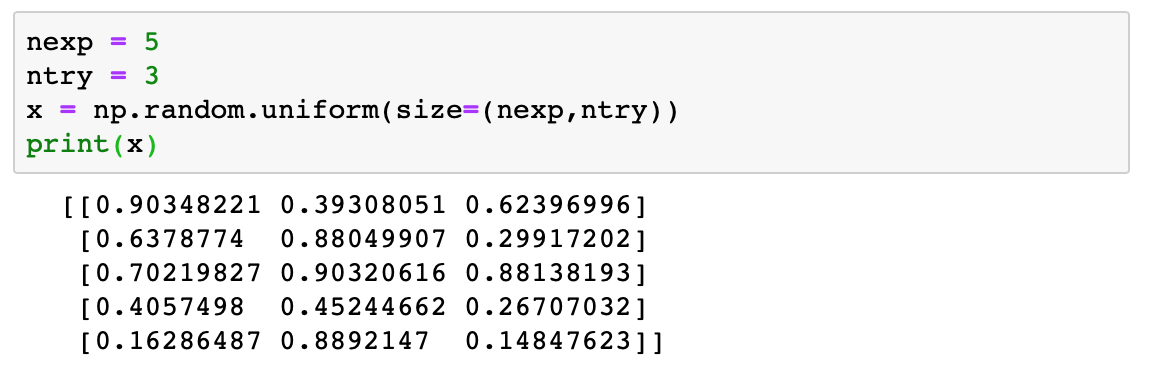
\includegraphics[width=0.85\textwidth]{figs/labs/distributions/makearray.png} \\
This array associates a random value with each trial from each
experiment.  
\item Consider a trial successful if the randomly chosen value is less
  than $\epsilon$.  In this example, taking $\epsilon = 0.5$ and
  assuming 1 indicates success and 0 a failure, we obtain:
\begin{samepage}
\begin{verbatim}
[[0 1 0]
 [0 0 1]
 [0 0 0]
 [1 1 1]
 [1 0 1]]
\end{verbatim}
\end{samepage}
In the first simulated experiment, only the second trial was
successful.  In the second experiment, only the last trial successful.
And so on.

\item Next, count the number of trials that were successful in each experiment.  The result will be a 1-D array of length $n_{\rm exp}$.  Consider using the {\tt np.sum} function with the {\tt axis} parameter (If documentation is unclear to you, check the examples).    In this example, we obtain the array of outcomes $m$:
\begin{verbatim} 
[1 1 0 3 2]
\end{verbatim}
This is the outcome of our five simulated experiments.  The first
and second experiment have one out of three trials successful, the third
experiment had zero out of three trials successful, and so on.
\end{itemize}

Work through the example and make sure you see how each result follows
from the previous step.  Then implement and test your own version of
this algorithm in Scientific Python.  If you are an experienced
programmer, you should put your simulation into a function like:
\begin{verbatim}
    def throw_binomial(nexp,ntry,eps):
       x = np.random.uniform(size=(nexp,ntry))
       #...your simulation follows...    
\end{verbatim}

This will make your code much easier to manage, because you can simply
call this function each time you need to run your simulation, but it
is optional.  Cutting and pasting is also permissible.

When validating a numerical calculation, think hard about good test
cases.  For instance, if you only test with the value of $\epsilon =
0.5$, you won't catch a bug that mistakes success for failure.  Try a
few different test cases, with reasonably small values for $n_{\rm
  try}$ and $n_{\rm exp}$ and check your numerical simulation.
Boundaries often make a good check, for instance $\epsilon = 0$ and
$\epsilon = 1$.

Another effective validation strategy is to check known mathematical
relations using your simulation.  For instance, we know that the mean
value of a Binomial distribution is given by:
\begin{equation} \label{eqn:binom_mean}
\bar{m} = n_{\rm try} \cdot \epsilon
\end{equation}
and that the variance is given by:
\begin{equation} \label{eqn:binom_var}
\sigma^2 = n_{\rm try} \cdot \epsilon \, (1 - \epsilon)
\end{equation}
and so these predicted values, calculated from your parameters
$\epsilon$ and $n_{\rm try}$ can be compared to the mean and variance
of the outcome array $m$ from your simulation, calculated using the numpy functions {\tt np.mean} and {\tt np.var}.  A
comparison with $n_{\rm exp}=1000$, $n_{\rm try}=10$, and
$\epsilon=0.5$ should result in something like:\\
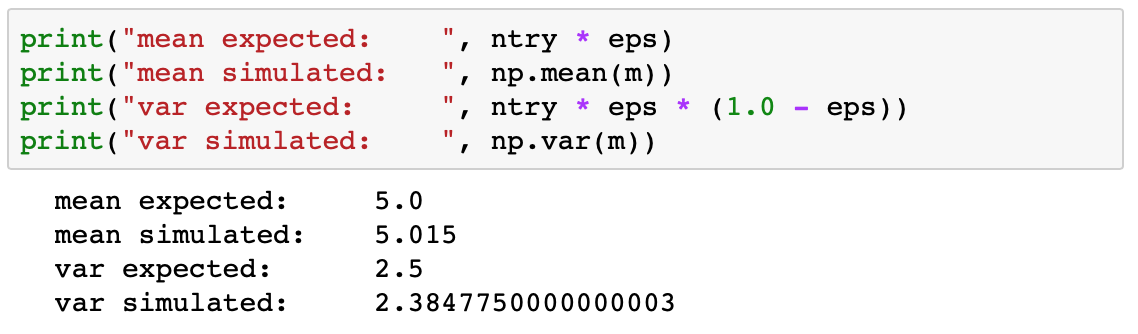
\includegraphics[width=0.8\textwidth]{figs/labs/distributions/validate.png}\\ 

\begin{plot}
Produce a large number of pseudo-experiments by setting $n_{\rm exp} =
1000$ and comment out any debugging print statements which will get
very long.  Pick two  well chosen test cases with different values of
$n_{\rm try}$ and $\epsilon$ and compare the expected and simulated
mean and variances. 
\end{plot}

The simulated values will fluctuate by a fractional amount
$1/\sqrt{n_{\rm exp}}$.  So for $n_{\rm exp} = 1000$, we expect the
expected and simulated values to agree within about $3\%$.

\begin{plot}
Increase the number of pseudo-experiments to $n_{\rm exp} = 100000$.
The agreement should improve to better than $1\%$.  Be certain to
print your test cases and the results in a clear way in your notebook.
\end{plot}

\section{Histogram for the Binomial Process}

We use histograms to represent the distribution of numerical data.  In
this case, our histogram simply reports the number of times each particular outcome
occurs.  Fill an output array $m$ with the simulated results of $n_{\rm exp} =
1000$ experiments each consisting of $n_{\rm try}=10$ trials with
success rate $\epsilon=0.25$.  There are eleven possible outcomes for
each of these experiments: $0,1,2,\ldots,10$.  We want to know how
often each of these outcomes occurred.

\begin{plot} Construct and plot a histogram from your simulated results in array $m$ using the 
{\tt np.histogram} function: \end{plot}
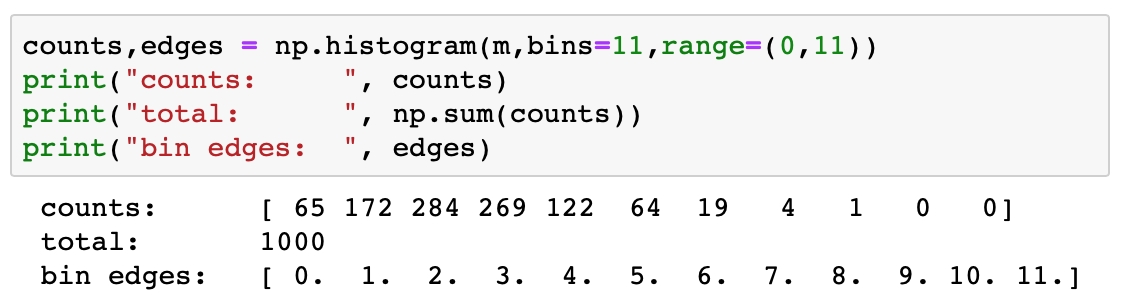
\includegraphics[width=0.8\textwidth]{figs/labs/distributions/makehist.png}\\ 
This calculates a histogram with eleven bins covering the range
from zero to eleven, and reports the number of outcomes from $m$ that
occur in each bin.  It returns two arrays, which we save as 
{\tt counts} and {\tt edges}.  We interpret the {\tt counts} array as
follows: the first entry tells us that 65 experiments had zero
successes, the second entry that 172 experiments had one success, the
third entry that 284 experiments had two successes, and so on.  The
exact values will vary each time you run the simulation, but in all
cases the sum across all bins will equal the total number of
experiments $n_{\rm exp} = 1000$.

Histograms are most often used to handle continuous data, so you
have to take a bit more care when using them to display discrete data
(integers) as we are doing here.  Consider the bin edges array {\tt
  edges} that was returned in this example:
\begin{verbatim}
   bin edges:   [ 0.  1.  2.  3.  4.  5.  6.  7.  8.  9. 10. 11.]
\end{verbatim}
which you will notice has length 12.  This is because the
array contains the {\bf edges} of eleven consecutive bins.  Technically the first bin
is the count of all outcomes in the range from zero (inclusive) to
just below one (exclusive).  The next bin is the count of all outcomes
in the range from one (inclusive) to just below two (exclusive).  In
this case, however, we are using discrete data, and so there are no entries with values like 1.73 to consider.
All the entries in the first bin are from experiments with the outcome
zero, while all the entries in the second bin are from the outcome
one.  The best way to plot this histogram, therefore, is
to associate each count with the leading bin edge, that is:\\
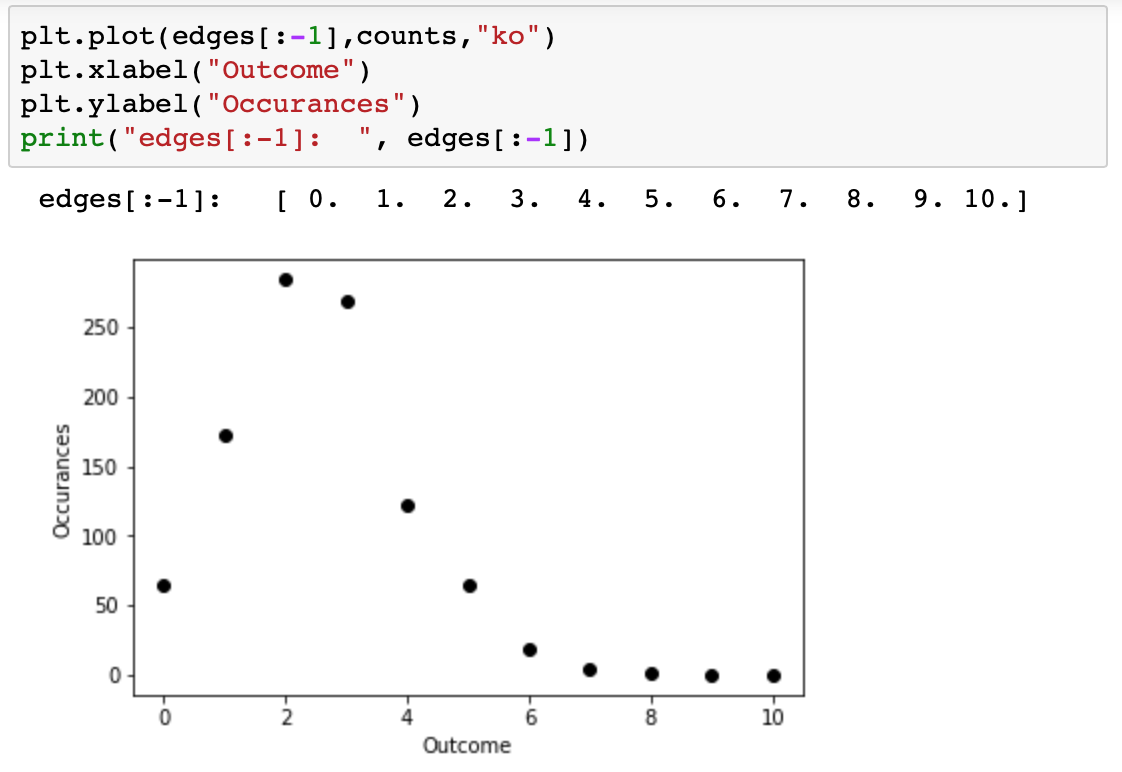
\includegraphics[width=0.8\textwidth]{figs/labs/distributions/plothist.png} \\
Notice the essential trick for plotting histogram with discrete data in integer bins is to use the slice {\tt edges[:-1]} of the bin edges data
\begin{verbatim}
   edges[:-1]:   [ 0.  1.  2.  3.  4.  5.  6.  7.  8.  9. 10.]
\end{verbatim}
as the $x$ values for plotting the occurrences of each outcome.  This
slice (all but the last entry) essentially throws out the superfluous
bin edge 11.  As we will see later, this trick only works for discrete
data in integer bins.  Notice that in resulting plot, we have the number of occurances
at each of the eleven possible outcomes correctly centered over the
numbers $0,1,2,\ldots,10.$

\section{Error Bars}

\begin{plot} Add error bars to your histogram and make a new plot.
\end{plot}
Run your simulation a few times and you will observe that the
simulated values fluctuate slightly each time you run your code.  But
how much should we expect these values to fluctuate?  If you consider
a single bin of your histogram in isolation, it contains a single
count $N$, which is itself the result of a simple counting experiment.
Counting experiments are described by the Poisson distribution.  Our
best estimate for the mean value $\lambda$ of this counting experiment
is simply our count $N$.  For the Poisson distribution the variance
$\sigma^2=\lambda$, and so we expect $\sigma = \sqrt{\lambda} =
\sqrt{N}$.  We expect each bin in our histograms to fluctuate by an
amount $\sigma$ which is the square root of the value of the bin.

To aid in interpreting histograms, it is useful to indicate the amount
we expect each bin to fluctuate by adding to the data point an ``error
bar'' with a length equal to the square root of the size of the number
of events in the
bin:\\ 
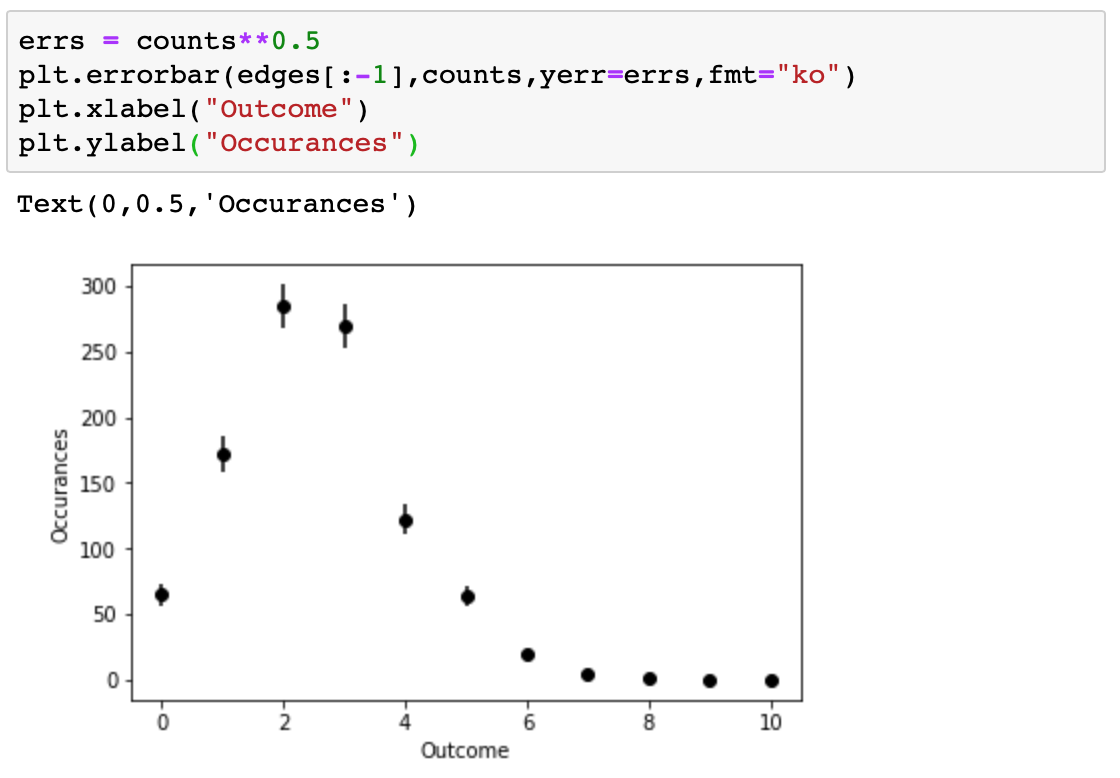
\includegraphics[width=0.8\textwidth]{figs/labs/distributions/plotbars.png}\\ 
This provides an intuitive visual indication for the size of the
statistical fluctuations associated with the counts reported by the
histogram.  Notice that the poorly named {\tt errorbar} function plots
{\em both} the data point and the error part, so it is a replacement
for the {\tt plot} function, not something you must call in addition.


\section{Comparison with Binomial PDF}

 Next we'd like to compare our Monte Carlo simulation with the PDF for
the binomial distribution.  We'll use the {\tt scipy.stats.binom.pmf}
function, which is the PDF for the discrete binomial distribution
available in Scientific Python.  This PDF is only non-zero at integer
values, so we'll simply evaluate it at each discrete occurrence,
i.e. the same slice {\tt edges[0:-1]} which we used to plot the
histogram:\\
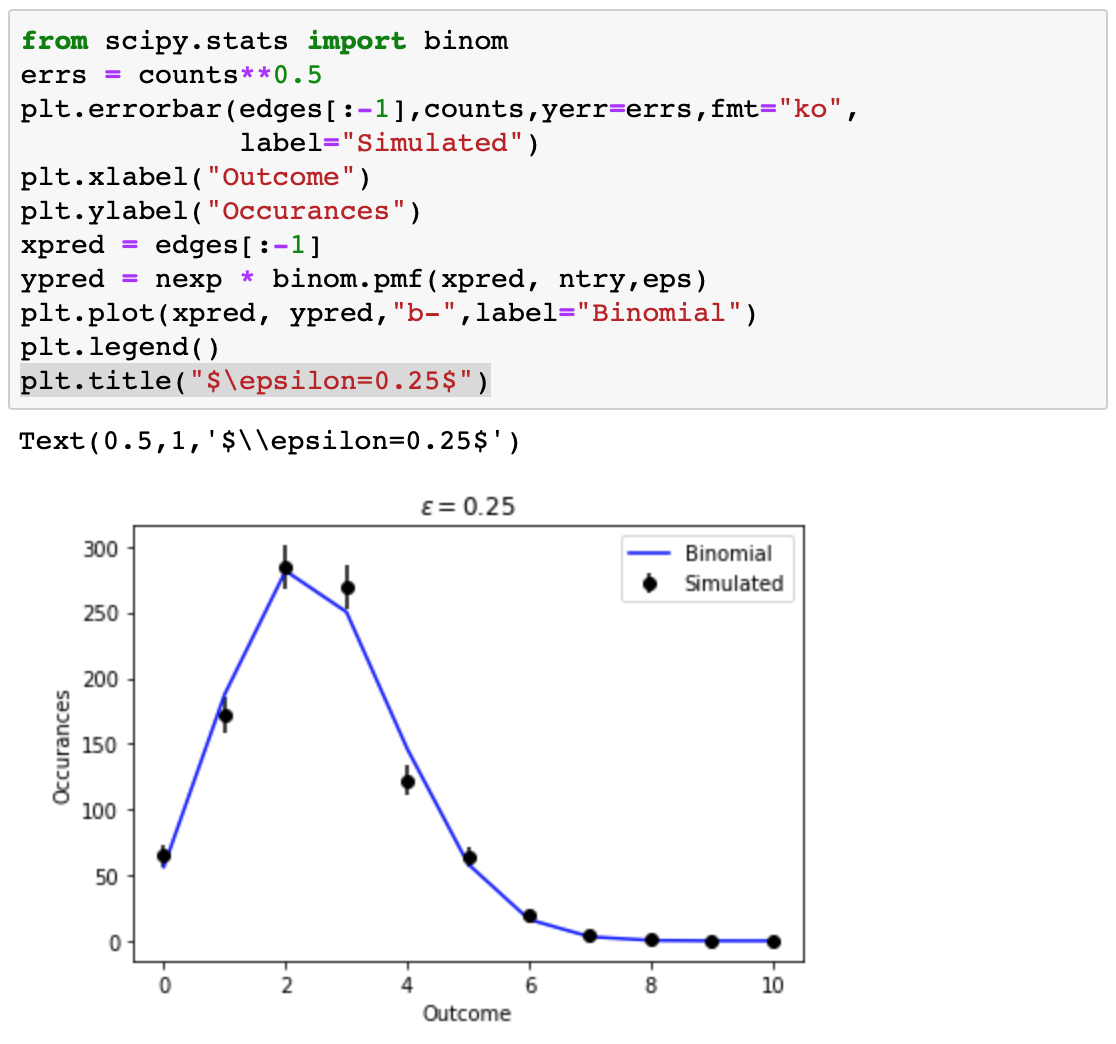
\includegraphics[width=0.85\textwidth]{figs/labs/distributions/compare.png}
\\ Notice that we scale the PDF by the number of experiments $n_{\rm
  exp}$.  The PDF is the expected frequency of each outcome for a
single experiment, but we are plotting the number of occurrences for
$n_{\rm exp}$ experiments.

\begin{plot} Compare the output of your Monte Carlo simulation
with the Binomial distribution PDF with $n_{\rm exp} = 1000$ and
$n_{\rm try} = 10$, and $\epsilon = 0.75$. See example for $\epsilon = 0.25$ in the plot above.
%and for three different values of $\epsilon$:
%0.25, 0.5, and 0.75.  For example, Plot 1 should look like the plot above. 
\end{plot}


\section{The Poisson Limit}

The Poisson distribution follows from the Binomial distribution in the
limit that $n_{\rm try} \to \infty$.  Recall that the mean value of
the Poisson distribution is $\bar{m} = \epsilon \, n_{\rm try}$.  If
we kept the success rate $\epsilon$ as a parameter, than any finite
value of $\epsilon$ would cause the mean of the distribution to diverge to infinity.
If instead we hold the new parameter $\lambda$ constant, and set:
\begin{displaymath}
\epsilon = \frac{\lambda}{n_{\rm try}}
\end{displaymath}
we see that $\epsilon \to 0$ as $n_{\rm try} \to \infty$ and the mean
of the Poisson distribution remains at the fixed value $\lambda$.

We'll explore this limit numerically simply by taking $n_{\rm try}$ to
the large (but finite) value of 1000.  Re-run your Monte Carlo
simulation using the parameters $n_{\rm try} = 1000$, $n_{\rm exp} =
1000$, and $\epsilon = \lambda / n_{\rm try}$.  For now, take $\lambda
= 2.0$.  Instead of the Binomial distribution, compare your simulation to the Poisson distribution PDF
using the {\tt poisson.pmf} function:
\begin{verbatim}
from scipy.stats import poisson
xpred = edges[:-1]
ypred = nexp * poisson.pmf(xpred, lamb) 
\end{verbatim}
Note that the first argument of the {\tt pmf} function is the array of
positions to evaluate the function at, while the second is the Poisson
parameter $\lambda$.  Also note that sadly {\tt lambda} is a reserved word
in python, and so you cannot use it as a variable name.

\begin{figure}[htbp]
\begin{center}
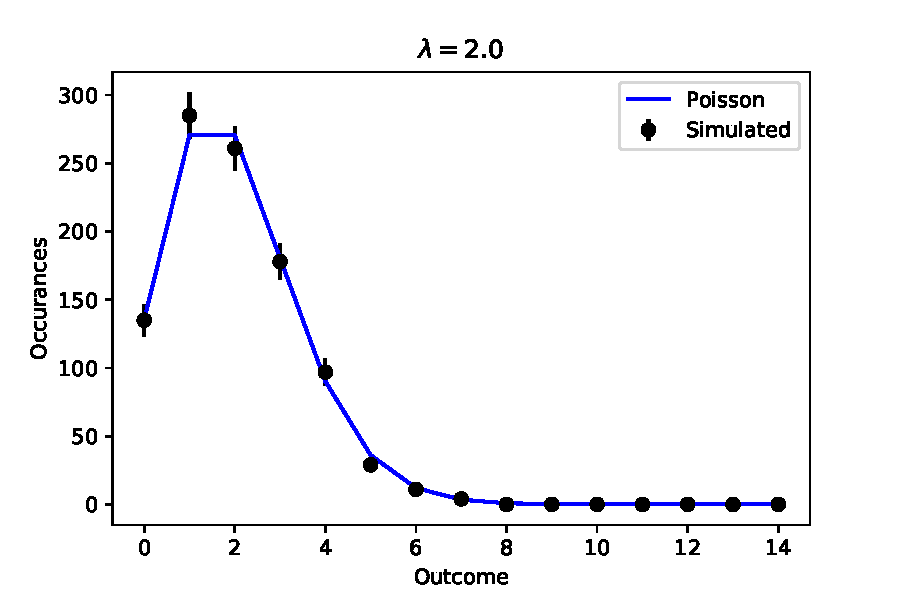
\includegraphics[height=0.22\textheight]{figs/labs/distributions/poisson.pdf}
\end{center}
\caption{\label{fig:poisson} Example of the expected result for the Monte Carlo simulation data in comparison to the Poisson PDF for for $\lambda=2$. }
\end{figure}

\begin{plot} In the Poisson limit, compare the output of your Monte Carlo simulation to the Poisson PDF
for $\lambda=5.2$.
%for two different values of $\lambda$:  2.0, 5.2.  
Plot the histogram with 15 bins for the outcomes: 0,1,2,3,...,14.  
An example for $\lambda=2$ is shown in Fig.~\ref{fig:poisson}.
\end{plot}

%Using {\tt np.mean} and {\tt np.var}, check that mean and variance of
%your distributions is as you expect in each case, and record the
%results in your log book.

\section{The Gaussian Limit}

\begin{figure}[htbp]
\begin{center}
\begin{tabular}{cc}
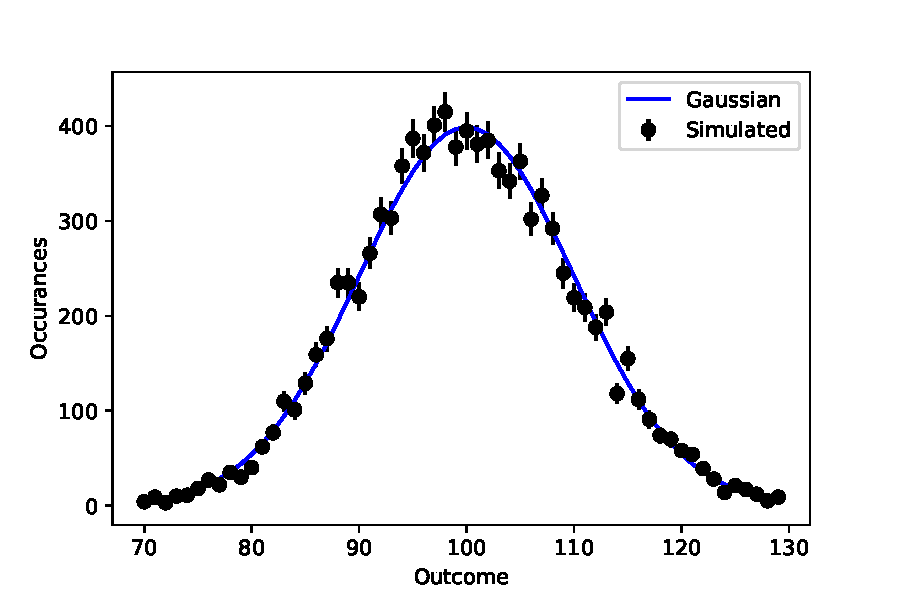
\includegraphics[height=0.22\textheight]{figs/labs/distributions/gauss_finebins.pdf} &
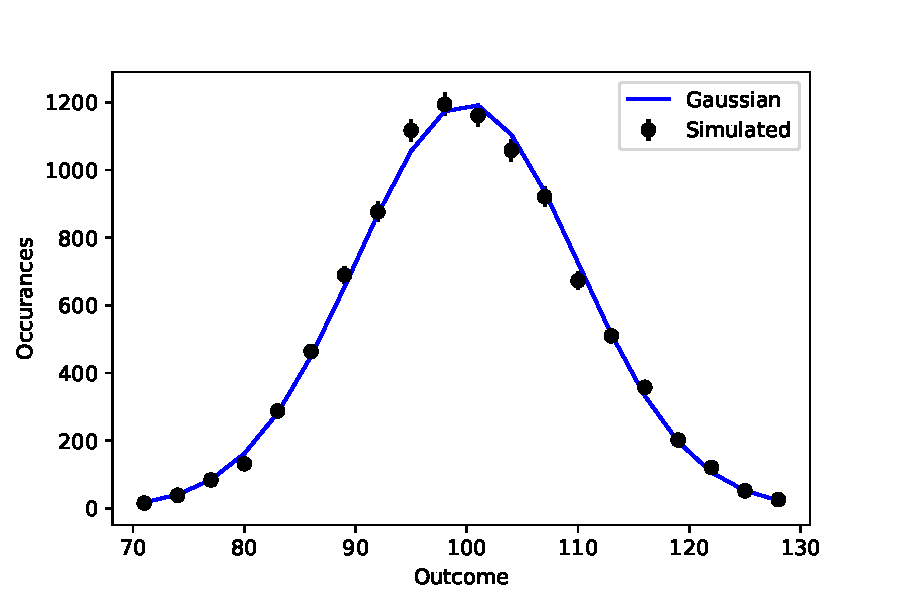
\includegraphics[height=0.22\textheight]{figs/labs/distributions/gauss.pdf} \\
(a) & (b) \\
\end{tabular}
\end{center}
\caption{\label{fig:gauss} Example of the expected result for the Monte Carlo simulation data in comparison to the Gaussian PDF for $\lambda=100$. }
\end{figure}

As the mean value $\lambda$ of the Poisson distribution gets larger,
the Poisson distribution resembles the Gaussian distribution.  We will
simulate this numerically by taking our Monte Carlo simulation in the
Poisson limit, as above, with $\lambda = 100$.  Initially use
integer bins inclusively in the range 70 to 130, e.g.:
\begin{verbatim}
counts,edges = np.histogram(m,bins=60,range=(70,130))
\end{verbatim}
and compare with the Gaussian (also called normal) distribution PDF, e.g.:
{\tt scipy.stats.norm.pdf} function:
\begin{verbatim}
from scipy.stats import norm
xpred = edges[:-1]
ypred = nexp * norm.pdf(xpred, loc=lamb, scale=lamb**0.5). 
\end{verbatim}

\begin{plot} Set the parameter {\tt loc} to the mean value, and the parameter {\tt
  scale} to $\sigma$.  Recall that in the Poisson limit $\sigma^2 =
\lambda$, which is why we set {\tt scale=lamb**0.5} in the example.
This should reproduce the plot in Fig.~\ref{fig:gauss}a. \end{plot}

You should see that 60 bins is rather unwieldy.  We'll reduce the number
of bins, but that's actually a bit more complicated than you might
expect: non-integer bins with discrete data is about the most
challenging binning you can tackle.  You'll have to do the following:
\begin{itemize}
\item While keeping the range of 70 to 130, set the number bins to {\tt bins=20} when filling your histogram.
\item Our trick to use edges[:-1] will no longer work, since now the data for each bin is associated with a range of values in the bin.  Each bin is now 3 integers wide. If we live this as is, edges[:-1] will position the x value of the bin at its leading edge: 70, 73, 76 , ......  and the data will be plotted with an observable bias.  For continuous data, we often simply use the middle of the bin:
\begin{verbatim}
cbins = (edges[:-1] + edges[1:])/2.  
\end{verbatim}
This would position the x value of the bins at 71.5, 74.5. 77.5, ..... and that seems more reasonable choice. 
In this specific case of discrete data which doesn't extend  all the way to the right edge this is still slightly biased. The first bin in our example represents the count of all outcomes in the range from 70 (inclusive) to below 73 (exclusive). So its center should be at 71.  To be precise for this specific case, the x position we should use for plotting the contents of each bin is:
\begin{verbatim}
cbins = (edges[:-1] + edges[1:] -1 )/2 
\end{verbatim}
\item The normalization of the PDF to the data now requires an additional scale factor to account for the wider bins (which integrate more probability).  You need to scale by an additional factor of 3 to account for the fact that each bin is 3 integers wide.
\end{itemize}

\begin{plot} Using the techniques described above, reproduce Fig~\ref{fig:gauss}b, which shows that the Binomial distributions becomes a Gaussian distribution as the mean value of the distribution becomes large. \end{plot}
























